\documentclass[12pt,a4paper,twocolumn,titlepage]{beamer}
\usepackage{beamerthemeAntibes}%tema beamer
\usepackage[utf8x]{inputenc}
\usepackage{ragged2e}%para usar \justifying
\usepackage[brazil]{babel}
\usepackage{ucs}
\usepackage{amsmath}
\usepackage{amsfonts}
\usepackage{amssymb}
\author{Josué Crispim}
\title{Estratégias computacionais para a busca de genes alvos de \textit{ dehydration responsive binding proteins} (DREBs) na soja}

\begin{document}
	\frame{\titlepage}
	
%Apresentar conteudo em cada transição de assunto
\AtBeginSection[]
{
   \begin{frame}
       \frametitle{Sumário}
       \tableofcontents[currentsection]
   \end{frame}
}

\section{Transcrição}
\frame{ \justifying
     \frametitle{Início da regulação de um gene}
     \begin{itemize}
		\item Um dos primeiros passos para a expressão de um gene é a transcrição.
		\item Onde diversos fatores podem influenciar a indução ou a repressão da expressão.		     
     \end{itemize}
%O primeiro passo na expressão de um gene é a transcrição. No processo de transcrição muitos fatores internos ou externos, na célula, podem influenciar induzindo ou reprimindo a expressão dos diversos genes codificados no genoma do organismo. Fatores externos desafiantes, como estresses bióticos e abióticos, até mecanismos moleculares intrínsecos podem desencadear, direta ou indiretamente, a ativação da expressão gênica espaço-temporal.
}

\frame{ \justifying
	\frametitle{Ácidos nucleicos}
	\begin{itemize}
		\item Os ácidos nucleicos são importantes moléculas que contem o material genético da célula.
		\item Uma analogia de sistemas biológicos com sistemas de computadores é pensar nos ácidos nucleicos como um código objeto de um programa, onde este código é descifrado pelo o sistema operacional (a célula) que irá tomar as devidas ações. No caso de células a ação é a produção de proteínas.
	\end{itemize}
% Na transcrição de um gene há diversos atores que trabalham em conjunto mas cada um com tarefaz específicas, uns desses autores são os ácidos nucleicos.
}

\frame{ \justifying
	\frametitle{Ácidos nucleicos}
	\begin{itemize}
		\item A composição química dos ácidos nucleicos é: um açúcar, uma base nitrogenada e um ácido fosfórico.
		\item Eles são ligados formando uma sequência linear.
	\end{itemize}
}

\frame{ \justifying
	\frametitle{Ácidos nucleicos}
\begin{figure}[htb!]
    \centering
    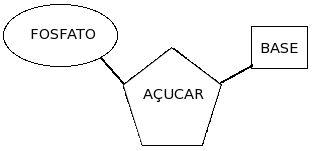
\includegraphics[scale=0.7]{./imagens/componentes_nucleotideo.png}
    \caption{Componentes de um nucleotídeo}
    \label{fig:nucleotideo}
\end{figure}
}

\frame{ \justifying
	\frametitle{Ácidos nucleicos}
\begin{figure}[htb!]
    \centering
    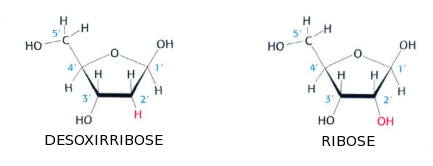
\includegraphics[scale=0.7]{./imagens/tipos_acucar.png}
    \caption{Tipos de açúcar encontrados nos ácidos nucleicos. \cite[Adaptada]{Berg2007})}
    \label{fig:tipos_acucar}
\end{figure}
}

\frame{ \justifying
	\frametitle{Ácidos nucleicos}
\begin{figure}[htb!]
    \centering
    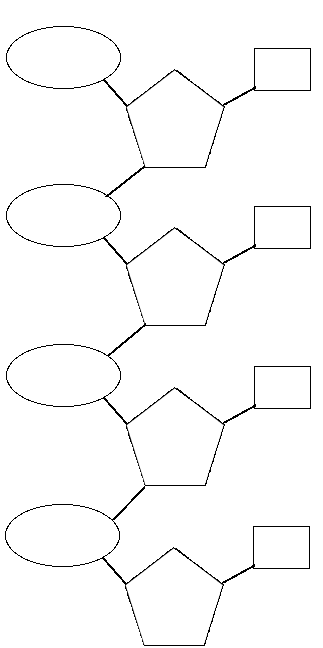
\includegraphics[scale=0.3]{./imagens/sequencia_nucleotideo.png}
    \caption{Sequência linear de nucleotídeos ligados}
    \label{fig:sequencia_nucleotideo}
\end{figure}
}


\frame{ \justifying
	\frametitle{Ácidos nucleicos}
	Existem dois tipos de ácidos nucleicos:
	\begin{enumerate}
		\item Ácido desoxirribonucleico (DNA)
		    \begin{itemize}
		    	\item açúcar: desoxirribose
		    	\item bases: A,\textbf{T}, G e C
		    	\item estrutura: duas sequências complementares pareadas formando um helicoide
		    \end{itemize}
		\item Ácido ribonucleico (RNA)		
		    \begin{itemize}
		    	\item açúcar: ribose
		    	\item bases: A, \textbf{U}, G e C
		    	\item estrutura: única sequência de nucleotídeos
		    \end{itemize}
	\end{enumerate}
	
}
	
\frame{ \justifying
	\frametitle{Ácidos nucleicos}
\begin{figure}[htb!]
    \centering
    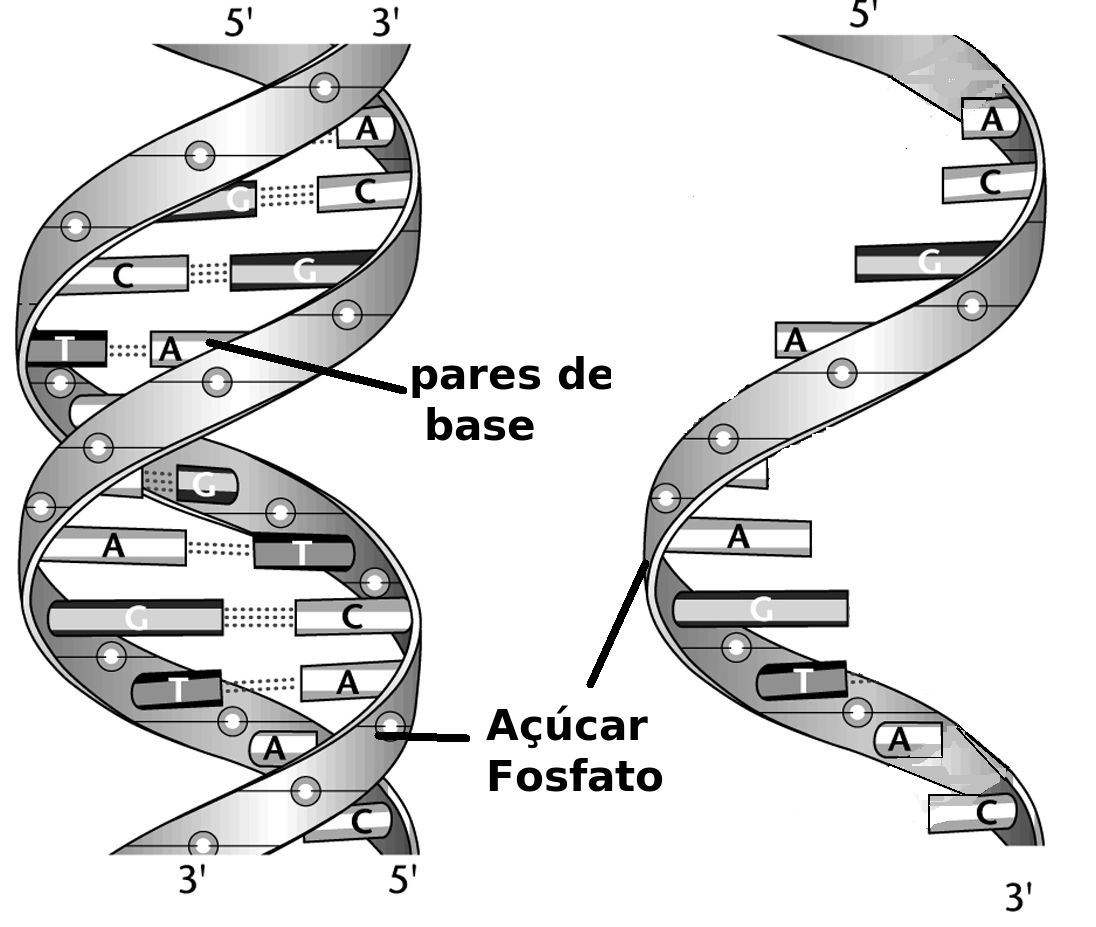
\includegraphics[scale=0.7]{./imagens/estrutura_DNA_RNA.jpg}
    \caption{Estrutura do DNA e RNA. \cite[Adaptada]{Higgs2005}}
    \label{fig:estrutura_DNA_RNA}
\end{figure}
}

\frame{ \justifying
	\frametitle{Transcrição}
	\begin{itemize}
		\item A transcrição consiste na formação do RNA a partir do DNA.
		\item É feita uma cópia exata de um segmento de DNA.
		\item Parte do RNA formado será usado na síntese de proteínas.
%		\item Os genes contém as informações que especificam um tipo de proteína.
		\item Todo esse processo é conhecido como dogma central.
	\end{itemize}
}

\frame{ \justifying
	\frametitle{Transcrição}
\begin{figure}[htb!]
    \centering
    
\includegraphics[scale=0.7]{./imagens/passo_expresscao_genica.png}
    \caption{Principais passos da expressão de genética}
    \label{fig:passo_expresscao_genica}
\end{figure}
}

\frame{ \justifying
	\frametitle{Transcrição}
		\begin{itemize}
			\item Para que ocorra a transcrição é necessário a ação de uma enzima chamada RNA-polimerase.
			\item Ela se conecta no DNA juntamente com fatores de transcrição gerais (formando um complexo)
			\item A RNA-polimerase se movimenta na direção 5' $\rightarrow$ 3' formando o RNA.
		\end{itemize}
}

\frame{
	\frametitle{Transcrição}
		\begin{figure}[htb!]
		    \centering
		    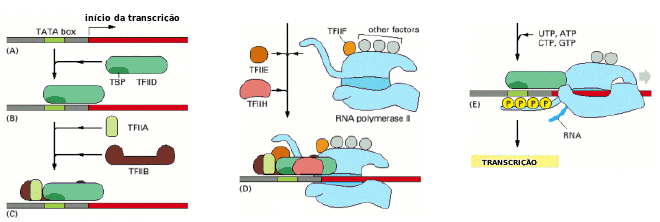
\includegraphics[scale=0.65]{./imagens/complexo_RNA-polimerase.png}
		    \caption{RNA polimerase e os fatores de transcrição gerais \cite[Adaptada]{Alberts2002} }
		    \label{fig:complexo_RNA-polimerase}
		\end{figure}
}

\frame{ \justifying
	\frametitle{Transcrição}
\begin{figure}[htb!]
    \centering
    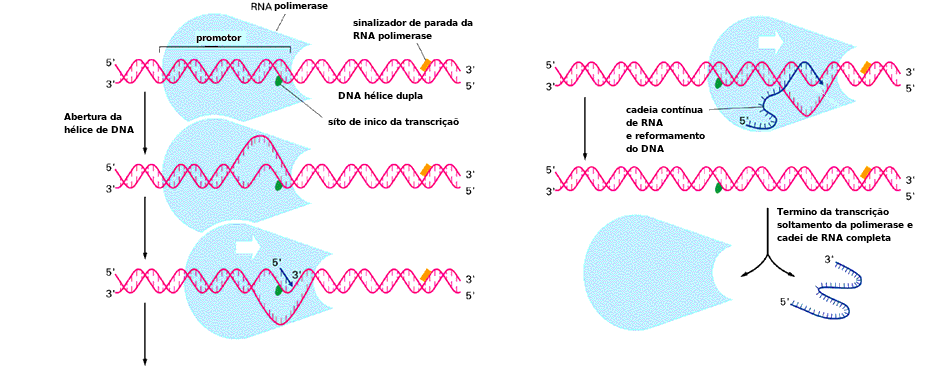
\includegraphics[scale=0.45]{./imagens/RNAPOLII.png}
    \caption{Formação do RNA através da RNA polimerase \cite[Adaptada]{Higgs2005}}
    \label{fig:RNAPOLII}
\end{figure}
}
\section{Elementos regulatórios e Fatores de transcrição}

   \frame{\justifying
    \frametitle{Região reguladora}
      \begin{itemize}            
        \item Cada gene tem uma região regulatória, geralmente de 100-1000 pares de bases acima do local de início da transcrição.
		\item Dentro dela estão os elementos regulatórios.
	  \end{itemize}
	}
	
   \frame{\justifying
    \frametitle{Elementos regulatórios}
       \begin{itemize}            
        	\item	São pequenas sequências de DNA localizadas a uma distância aproximada de -50 pares de base do local de início da transcrição na região promotora de um gene (figuras \ref{fig:promotores_noDNA} e \ref{fig:localizacao_TFBS}).

			\item O tamanho aproximado dos elementos regulatórios varia entre 5 a 20 nucleotídeos.

			\item Cada elemento regulatório é específico a um fator de transcrição.
	   \end{itemize}
   }
   
\frame{
     \frametitle{Elementos regulatórios}
\begin{figure}[htb!]
    \centering
    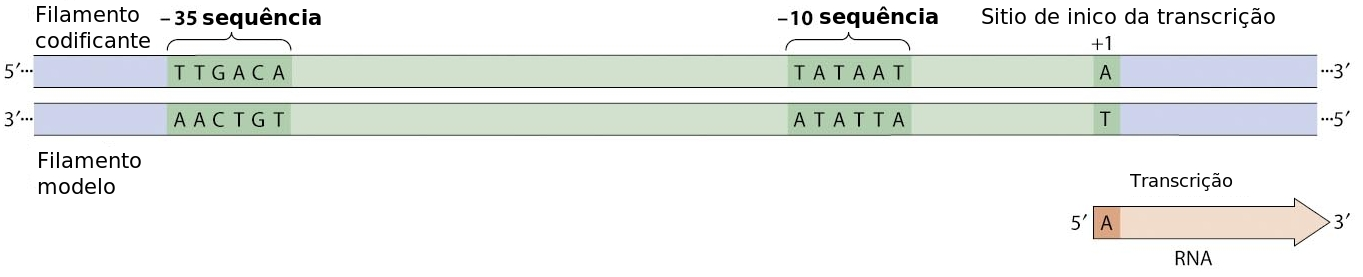
\includegraphics[scale=0.5]{./imagens/promotores_noDNA.jpg}
    \caption{Região promotora e as sequências consenso}
    \label{fig:promotores_noDNA}
\end{figure}
}

\frame{
     \frametitle{Elementos regulatórios}
    \begin{figure}[htb!]
    \centering
    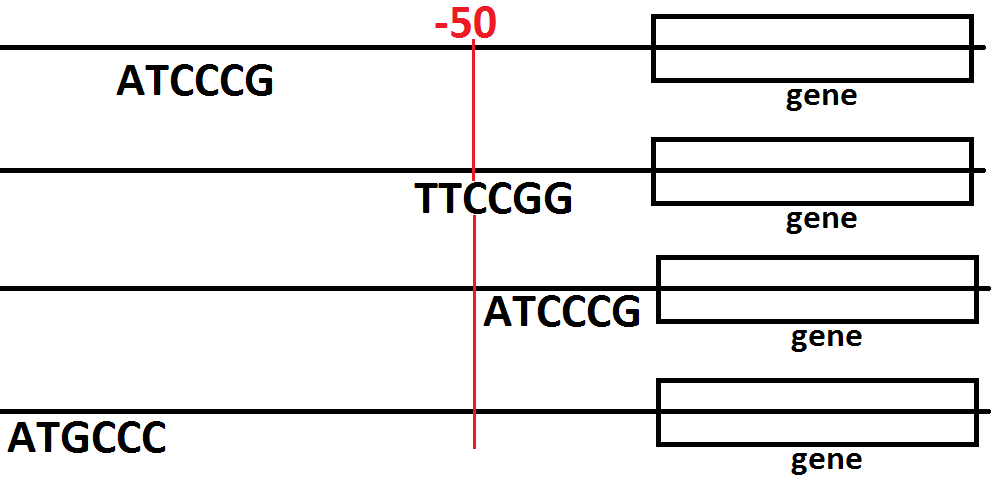
\includegraphics[scale=0.4]{./imagens/localizacao_TFBS.png}
    \caption{Localização aproximada dos elementos regulatórios}
    \label{fig:localizacao_TFBS}
    \end{figure}     
}

\frame{\justifying
     \frametitle{Fatores de Transcrição}
     Proteínas "especiais" chamadas de  \textbf{fatores de transcrição} (TF do inglês \textit{transcription factor binding site}) se ligam nos elementos regulatórios, contribuindo para o início da transcrição de um gene. Podem ser separados em fatores de transcrição gerais e específicos. (figuras \ref {fig:complexo_RNA-polimerase} e \ref{fig:TF_lingando_no_DNA}).

}

\frame{
     \frametitle{Fatores de Transcrição}
    \begin{figure}[htb!]
    \centering
    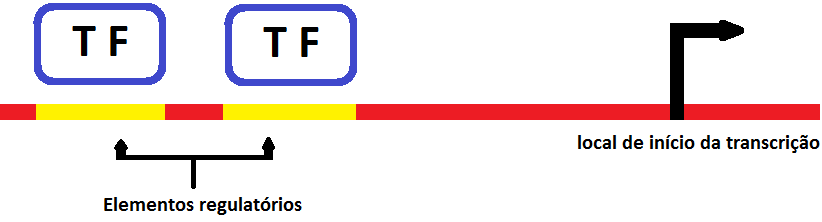
\includegraphics[scale=0.5]{./imagens/TF_lingando_no_DNA.png}
    \caption{Localização aproximada dos elementos regulatórios}
    \label{fig:TF_lingando_no_DNA}
    \end{figure}     
}

\frame{\justifying
	\frametitle{Funcionalidade na célula}
	Os elementos regulatórios juntamente com os fatores de transcrição funcionam como mecanismos de respostas a diversos estímulos, como:
	\begin{itemize}
		\item estímulos internos.
		\item estresses abióticos.
		\item estresses bióticos.				
	\end{itemize}
%    Estresses abióticos e bióticos influenciam negativamente na sobrevivência e na larga produção de grãos.
%	Existem elementos regulatórios que são ativados em resposta a estímulos como mudanças hormonais internamente em um organismo, ou externamente como: estresses abióticos que são causados por fatores não vivos como a alteração de temperatura e mudança climática, ou estresses bióticos causados por organismos vivos como bactérias, vírus, parasitas e insetos. Com a ativação do elemento regulatório ocorrera a expressão do gene, que o elemento regula, o gene será transcrito no RNA que posteriormente será traduzido, gerando proteínas para suprir as necessidades do organismo.
}

\frame{\justifying
	\frametitle{Funcionalidade na célula}
	Com a ativação de um elemento regulatório ocorre a expressão de um gene, que o elemento regula, o gene será transcrito no RNA que posteriormente será traduzido, gerando proteínas para suprir as necessidades do organismo.
}

\section{Dehydration Responsive Binding Proteins(DREBs)}
\frame{ \justifying
	\frametitle{DREBs}
	São fatores de transcrição que agem na célula, quando está é estimulada por um estresse abiótico como:
	\begin{itemize}
		\item seca
		\item alta salinização
		\item baixas temperaturas.
	\end{itemize}
}

\frame{\justifying
	\frametitle{DREBs}
	O entendimento dos DREBs na regulação de um gene é de grande importância para o desenvolvimento de plantas tolerantes a estresses.
}
\section{Busca de elementos regulatórios}

   \frame{\justifying
    \frametitle{Busca por padrões}
    	\begin{itemize}
    		\item A busca por elementos regulatórios remete a busca por padrões em uma \textit{string}.
    		\item Dado um padrão de DNA, encontrar sequências candidatas é simples, mas diferenciar sítios reais dos não reais é difícil.
    		\begin{itemize}
				\item Um fator de transcrição específico utilizado na expressão de um determinado gene, pode não ser o mesmo para a expressão de outro gene. Entretanto um único também TF pode regular múltiplos genes.
% Experimentos com microarray mostraram que, quando um gene X não é expresso, outros 20 não são expressos, uma vez que o gene X codifica proteinas reguladoras TFs, o 20 genes não expressos são regulados pelos TFs do gene X. 		 
				\item Essa especificidade torna os elementos regulatórios em sequências que não são consenso.

%Um fator de transcrição específico utilizado na expressão de um determinado gene, pode não ser o mesmo para a expressão de outro gene. Por exemplo o conjunto de fatores de transcrição de uma célula óssea no organismo humano, pode ter fatores diferentes do conjunto de TFs de uma célula do figado, uma vez que essas diferentes células podem precisar de diferentes proteínas. Essa especificidade torna os elementos regulatórios em sequências que não são consenso, em consequência os elementos regulatórios não seguem um padrão.	
	    	
	    		\item Pelo fato que muitos elementos regulatórios são usualmente degenerados, sofrem mutações, deleção ou inserção.	
    		\end{itemize}
    	\end{itemize}
	}
	
   \frame{\justifying
    \frametitle{Um exemplo da degeneração}
		\begin{figure}[htb!]
		    \centering
		    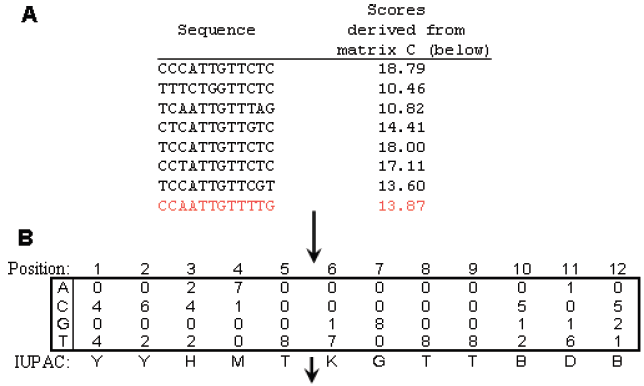
\includegraphics[scale=0.5]{./imagens/ET_caso_element1.png}
		    \caption{Oito conhecidos elementos regulatórios da \textit{Saccharomyces cerevisiae}, a pontuação esta de acordo com a PWM em C}
		    \label{fig:ET_caso_element1}
		\end{figure}		
	}	

   \frame{\justifying
    \frametitle{Um exemplo da degeneração}
		\begin{figure}[htb!]
		    \centering
		    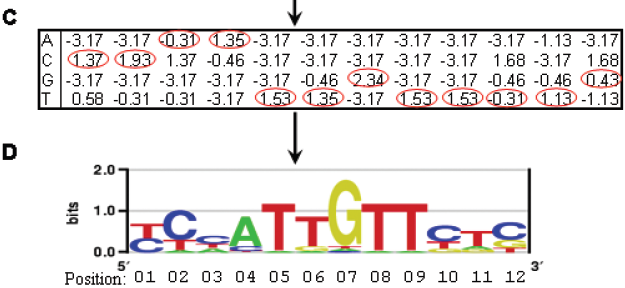
\includegraphics[scale=0.5]{./imagens/ET_caso_element2.png}
		    \caption{Matriz de peso das sequências alinhadas e a representação logo da sequência}
		    \label{fig:ET_caso_element2}
		\end{figure}		
	}	

   \frame{ \justifying
    \frametitle{Um exemplo da degeneração}
		Os valores da matriz de peso mostrada em C são obtidos calculando:
		$ \log_{2}(f_{i,j}/P_{i})$, onde $f_{i,j}$ é a frequência da base $i$ na posição $j$. Este valor pode ser obtido dividindo o valor da célula da matriz pelo numero de sítios na posição (p.e $f_{C,1} = f_{T,1} = 4/8 = 0.5$). E $P_{i}$ é a probabilidade de encontrar uma base na posição $i$, que é $P_{A} = P_{T} = 0.32$, e $P_{C} = P_{G} = 0.18$ (valor correspondente ao genoma do \textit{S.cerevisiae}).
	}	

	
%A busca por padrão pode ser descrita como, dado um conjunto de sequências de DNA e um tamanho L, o objetivo é identificar os padrões  mais significantes de tamanhos L. Como solução podemos gerar todos os possíveis padrões na sequência, então buscar o numero de ocorrência de cada padrão, reportando os que tiverem a maior frequência, como sendo os mais significativos. Este tipo de técnica garante bons resultados, até mesmo em padrões degenerados. Porém a procura por padrões com tamanhos grandes em um espaço de 4^L, têm um grande custo computacional, fazendo que se torne inviavel para buscas com L > 10. Para contornar este problema recorre-se ao uso de dados pré-processados, para diminuir o espaço e a busca se tornar menos custosa. Ou combinar a sobreposição de pequenos padrões encontrados para encontrar padrões maiores e mais complexos. Também, pode-se usar arvores sufixas que diminuem a complexidade e aumenta o tamanho de L. Estes tipos de abordagens também são conhecidas como abordagens de busca baseada em palavras.

%Nos metodos dirigidos pelas sequências o objetivo é encontrar a localização dos motifs e a PWM representativa usando apenas os dados da sequência, como a informação da localização dos motifs não é conhecida, está informação tem que ser aprendida. Para isto utiliza-se algoritmos de aprendizagem de maquina. Varios algoritmos foram propostos utilizando esta abordagem, como algoritmos gulosos, expectation-maximization (EM), Gibbs samplis entre outros.

%Outras abordagens  que vêm se destacando são: o de comparação entre os genomas para a busca dos elementos reguçatórios e da busca de modulos de elementos regualtórios.
	
   \frame{\justifying
    \frametitle{Busca de elementos regulatórios}
		\begin{itemize}
			   \item Para contornar esses problemas foram desenvolvidos vários algoritmos de busca de elementos regulatórios. Eles são classificados em três grupos:
				   \begin{enumerate}
						\item busca de em genes co-regulados
						\item busca em genes ortólogos 		   
						\item busca simultânea em genes ortólogos e co-regulados.
				   \end{enumerate}
		\end{itemize}
}

   \frame{\justifying
    \frametitle{Busca em genes co-regulados}
    	\begin{itemize}
			\item Genes que são regulados pelos mesmos conjuntos de fatores de transcrição.
    	\end{itemize}
    }

   \frame{\justifying
    \frametitle{Busca em genes co-regulados}
		\begin{figure}[htb!]
		    \centering
		    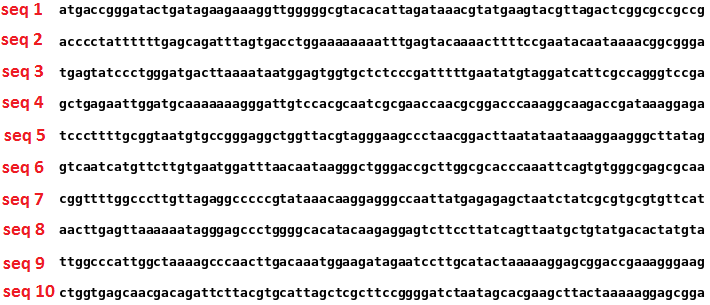
\includegraphics[scale=0.5]{./imagens/exe_element.png}
		    \caption{Diferentes sequências promotoras de uma mesma espécie}
		    \label{fig:exe_element}
		\end{figure}		
	}

   \frame{\justifying
    \frametitle{Busca em genes co-regulados}
		\begin{figure}[htb!]
		    \centering
		    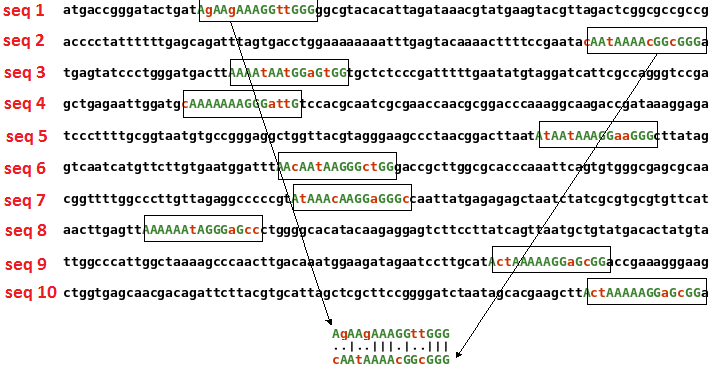
\includegraphics[scale=0.5]{./imagens/exe_element2.png}
		    \caption{Encontrado um padrão nas sequências}
		    \label{fig:exe_element2}
		\end{figure}		
	}


   \frame{ \justifying
    \frametitle{Oligo-Analysis}
    	Um dos métodos propostos para a identificação dos elementos regulatórios em genes co-regulados é o de \cite{Helden1998}. Os autores projetaram um algoritmo que detecta oligonucleotídios (um fragmento curto de DNA) sobre-representados na região promotora dentro de um grupo de genes co-regulados. O programa conta todas as ocorrências dos oligonucleotídios dentro do conjunto de sequências e estima a significância estatística.    	
	}
%	Como uma solução podemos gerar todos os possíveis padrões na sequência, então buscar o numero de ocorrência de cada padrão, reportando os que tiverem a maior frequência, como sendo os mais significativos.

   \frame{ \justifying
    \frametitle{Oligo-Analysis}
		Primeiramente foram calculadas as frequências esperadas $F_{e}\lbrace b \rbrace$ para cada oligonucleotídio $(b)$ de tamanhos de um a nove. Então determinada a ocorrência esperada para cada oligonucleotídio no conjunto de sequências promotoras com a formula $E(occ\lbrace b \rbrace) = F_{e}\{ b \}*T$ onde $T = 2xSx(L - w + 1)$, onde $w$ é a tamanho do oligonucleotídio; $S$ é o numero de sequências no conjunto; $L$ é o tamanho das sequências. O fator 2 é devido a soma de ocorrências é feita em ambos os filamentos de DNA.
	}
   \frame{ \justifying
    \frametitle{Oligo-Analysis}
		A significancia estatística é encontrada através da formula $P(ooc \lbrace b \rbrace = n) = \frac{T!}{(T -n)! x n!} x (F_{e}\{ b \})^n x (1 - F_{e}\{ b \})^(T -n) $. 
	}		
	\frame{ \justifying
    \frametitle{Oligo-Analysis}
	Depois que são encontrados os oligonucleotídios que são sobre-representados (que seguem um padrão) que têm grandes possibilidades de aparecerem em sequências promotoras, então são determinados nas sequências promotoras as posições que batem com os oligonucleotídios encontrados.
	% Probabilidade de encontra n ocorrências do oligonucleotifio b no conjunto de sequências, o com maior probabilidade é escolhido.
	}	
	\frame{ \justifying
    \frametitle{Oligo-Analysis}
	Este tipo de técnica garante bons resultados, até mesmo em padrões degenerados. Porém a procura por padrões com tamanhos grandes em um espaço de $4^L$, onde $L$ é o tamanho da sequência,tem um grande custo computacional, fazendo que se torne inviável para buscas com $L > 10$.	
	}

   \frame{\justifying
    \frametitle{Busca em genes ortólogos}
    	\begin{itemize}
			\item São genes \textit{homólogos} que foram separadas por um evento especial, fazendo que diferentes espécies tenham os mesmos genes.
    	\end{itemize}
%são genes/seqüências que derivaram de ancestrais comuns e conseqüentemente elas são conservadas e apresentam grande similaridade, por exemplo genes homólogos podem ser encontrados em dois diferentes organismos mas que derivaram do mesmo ancestral, por isso possuem o mesmo gene que é homologo entre esses dois organismos.     	
    }

   \frame{\justifying
    \frametitle{Busca em genes ortólogos}
		\begin{figure}[htb!]
		    \centering
		    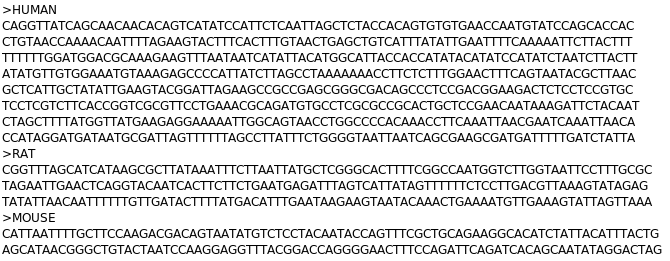
\includegraphics[scale=0.5]{./imagens/exe_seq.png}
		    \caption{Sequências de várias espécies}
		    \label{fig:exe_seq}
		\end{figure}		
	}
	
   \frame{\justifying
    \frametitle{Busca em genes ortólogos}
		\begin{figure}[htb!]
		    \centering
		    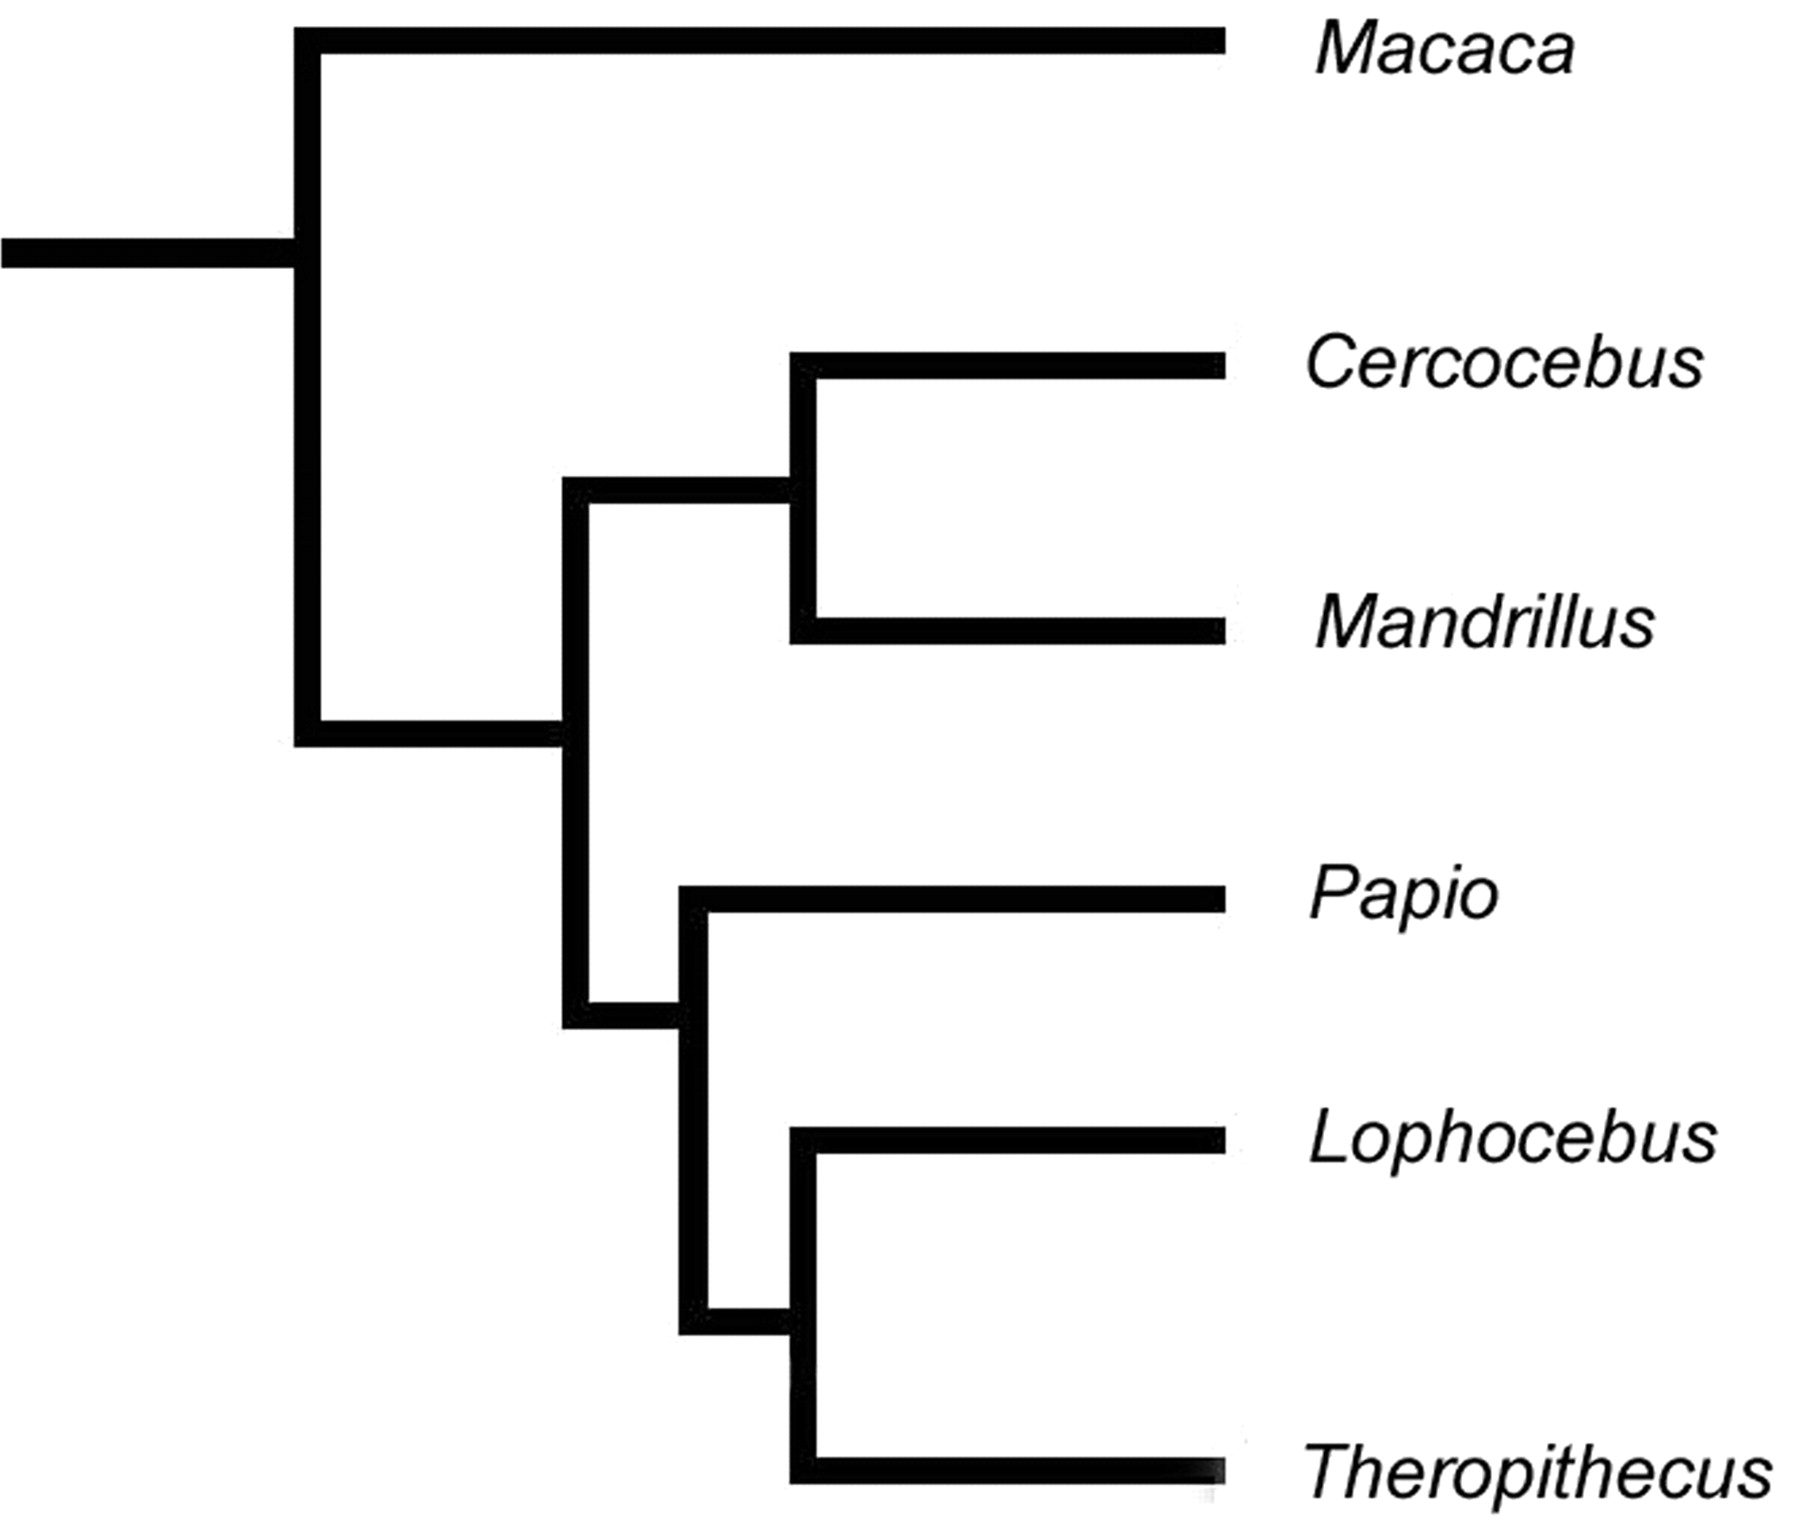
\includegraphics[scale=0.1]{./imagens/phy_tree.jpg}
		    \caption{Árvore filogenética}
		    \label{fig:phy_tree}
		\end{figure}		    	
	}

   \frame{\justifying
    \frametitle{FootPrinter}
    	\begin{itemize}
    		\item Este algoritmo \cite{Blanchette2002} tem como entrada uma a árvore filogenética e as sequências $s$ promotoras de várias espécies e o tamanho do elemento regulatório.
    		\item É calculado a menor pontuação de parcimônia da sub-árvore $d_{v}^* = \sum_{w \in C(v)} min_{t' \in \sum^{k}}(d_{w}^*(t')+d(t',t)$ até a raiz.
    		\item Então é gerado sequências randômicas $r$ que simulam a evolução das sequências $s$ mas sem pressão natural.
    		\item Calula-se a divergência entre $s$ e $r$.
    		\item $s$ e $r$ têm a mesma frequência de nucleotídeos.    		
    	\end{itemize}
	}
	
\section{Identificação de genes alvos de DREBs}
   \frame{\justifying
    \frametitle{Identificação de genes alvos de DREBs}
		Para identificar os genes alvos de DREBs \cite{Wang2009} criaram a seguinte estratégia:
		
		 	
	}
	
   \frame{\justifying
    \frametitle{Identificação de genes alvos de DREBs}
		\begin{figure}[htb!]
		    \centering
		    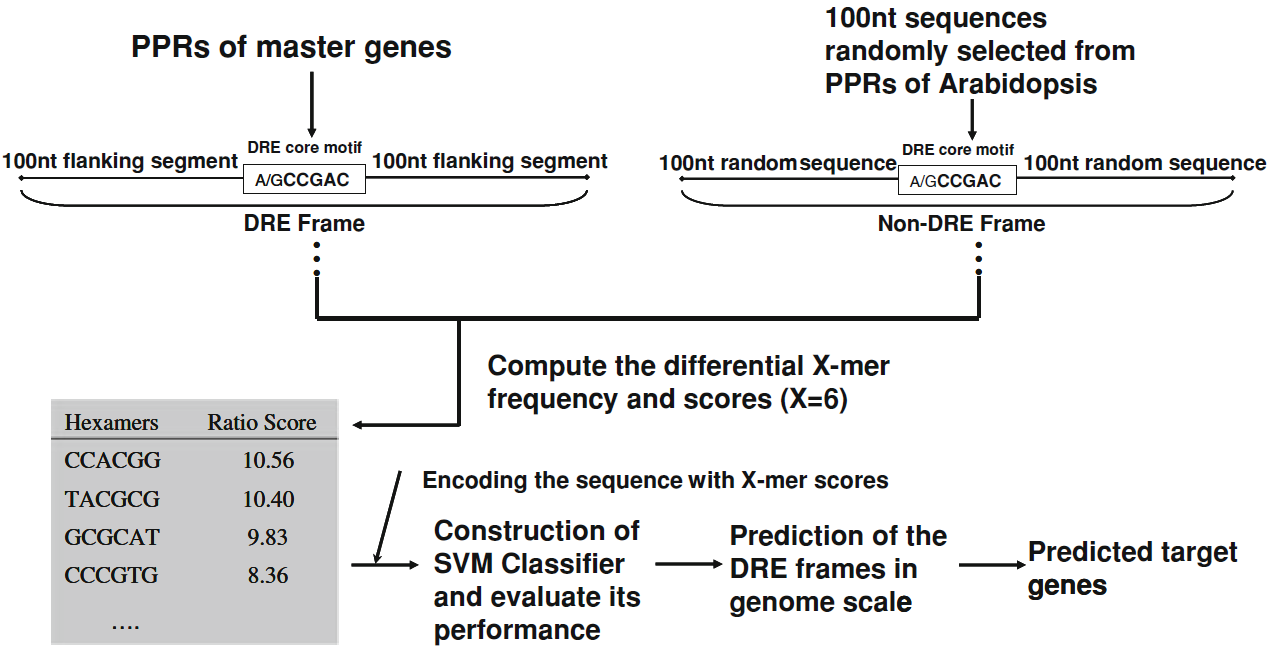
\includegraphics[scale=0.33]{./imagens/esq_DREB_find.png}
		    \caption{Busca DREBs}
		    \label{fig:esq_DREB_find}
		\end{figure}		    	
	}

   \frame{\justifying
    \frametitle{Identificação de genes alvos de DREBs}
		\begin{itemize}
			\item Achar a frequência em ambos os conjuntos $F{p}\{h\} e F_{n}\{h\}$.
			\item Calcular a razão $ R\{h\} = \frac{F{p}\{h\}}{F_{n}\{h\}}$
			\item Os DFS e nDFS recebem identificação de (+1) e (-1), respectivamente.
			\item SVM é treinada para distinguir entre DFS e nDFS.
		\end{itemize}	
	}
\section{Conclusão}
   \frame{\justifying
    \frametitle{Conclusão}
		Dos métodos apresentados para encontrar elementos regulatórios, em específico na soja
		seria mais adequado a utilização de métodos de genes co-regulados. Quanto aos DREBs, utilizar uma abordagem "reversa"(com os elementos regulatórios encontrar os genes alvos), também apresenta-se mais viável do ponto de vista da utilização da ferramenta.
	}

%\bibliographystyle{abnt-alf}
  \frame{
    \frametitle{Bibliografia}
\bibliography{bibliografia}
}
\end{document}